\chapter{Comparison with other ATLAS and CMS analyses}
\label{chap:summary_susy}

In this chapter we discuss the interplay of the searched presented in the previous two chapters and the 
wide program of \gls{susy} searched carried on by the \gls{atlas} and \gls{cms} collaborations. 

\section{Gluino pair production with decay through third generation squarks}

In the \gls{atlas} Collaboration only the multi-b analysis provides an interpretation for the Gbb model 
discussed in Chapter \ref{chap:strong_prod}.
Instead, in the cases of the Gtt model, a second analysis is interpreted to provide sensitivity  to this 
signal grid; this analysis, described in Ref \cite{Aaboud:2017dmy}, targets this model selecting final states with two same-charge 
leptons (electrons or muons), high jet multiplicity ($\geq$ six jets), one or two b-tagged jets and different \met selections 
(ranging from no \met selection to \met $>$ 200 GeV).

\begin{figure}[htbp]
	\centering
	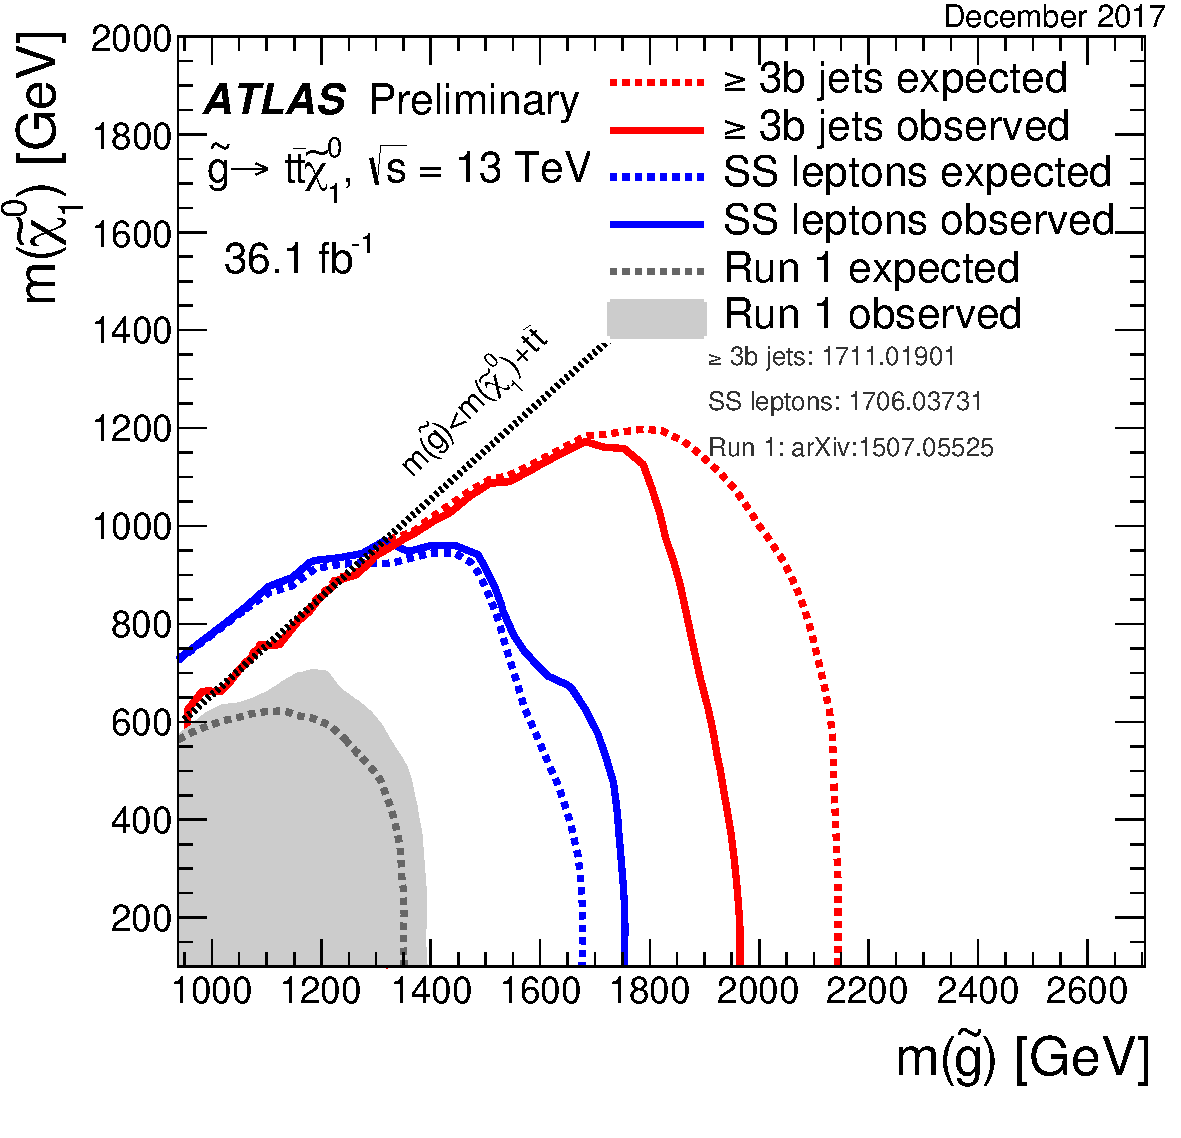
\includegraphics[width=0.52\textwidth]{figures/summary_plots/ATLAS_SUSY_Gtt.pdf}
	\caption{Exclusion limits at 95\% CL based on 13 TeV data in the (gluino, lightest neutralino) 
	mass plane for the Gtt simplified model where a pair of gluinos decays promptly via off-shell top 
	squarks to four top quarks and two lightest neutralinos. Theoretical signal cross section uncertainties are 
	not included in the limits shown. Figure from Ref. \cite{atlasSUSYSummary}.
	} 
	\label{fig:summary_atlas_Gtt}
\end{figure}

Figure \ref{fig:summary_atlas_Gtt} shows the overlay of the limits obtained with the multi-b analysis and with the two-same-charge-leptons analysis.
The latter has a very good sensitivity when the neutralino mass approaches the gluino mass,
limiting the amount of \met in the final state.
This analysis considers also signal models where the mass difference between the gluino and the neutralino 
is not enough to produce two on-shell top quarks and one of them is off-shell; this is why the limit extends above 
the "diagonal" where $m(\tilde{g}) = m(\ninoone) + 2 m(t)$.


In the case of the \gls{cms} Collaboration, several analyses provide an interpretation for both the Gtt and 
the Gbb signal models, shown respectively in Figures \ref{fig:limits_Gtt_cms} and \ref{fig:limits_Gbb_cms}.
The \htmiss analysis \cite{Sirunyan:2017cwe} provides the best sensitivity for both models in the case of massless 
neutralino; this analysis performs a four-dimensional scan of zero-lepton events with at least two jets, binning them 
based on the scalar sum of the \pt of the signal jets in the event (\Ht), the negative vector sum of the jets (\htmiss), 
the number of jets and the number of b-jets. 

In the case of the Gtt model, for high gluino mass and intermediate neutralino mass the most sensitive analysis is
the 0-lepton analysis with reconstructed hadrinically decaying top quarks \cite{Sirunyan:2017pjw}, 
that builds several \glspl{sr} based on the number of jets, the number of b-jet, the number of reconstructed top quark 
candidates, \met, \Ht and \mttwo, a transverse-mass type variable designed to reduce the \ttbar background. 
For signal models with small mass difference between the gluino and the neutralino, the most sensitive analysis 
is also for \gls{cms} the same-sign analysis \cite{Sirunyan:2017uyt}, that selects events with two leptons with 
the same charge and builds several \glspl{sr} based on number of jets, number of b-jets, \met, \Ht, and \mt. 

The \mttwo analysis \cite{Sirunyan:2017kqq}, that uses 0-lepton events with high \mttwo,
 is the one most sensitive for Gbb models with high gluino mass 
and intermediate neutralino mass. 
The Gbb signal does not produce any prompt lepton, so in this case also when the neutralino mass approaches the kinematic 
limit it is a 0-lepton analysis that provides the best sensitivity: 
in the \alphat analysis \cite{Sirunyan:2018vjp}, all the \glspl{sr} are defined in the phase-space region 
with large \alphat, defined as the ration between the energy of the sub-leading jet and the transverse mass
between the leading and subleading jet. 

\begin{figure}[htbp]
	\centering 
	\subfigure[]{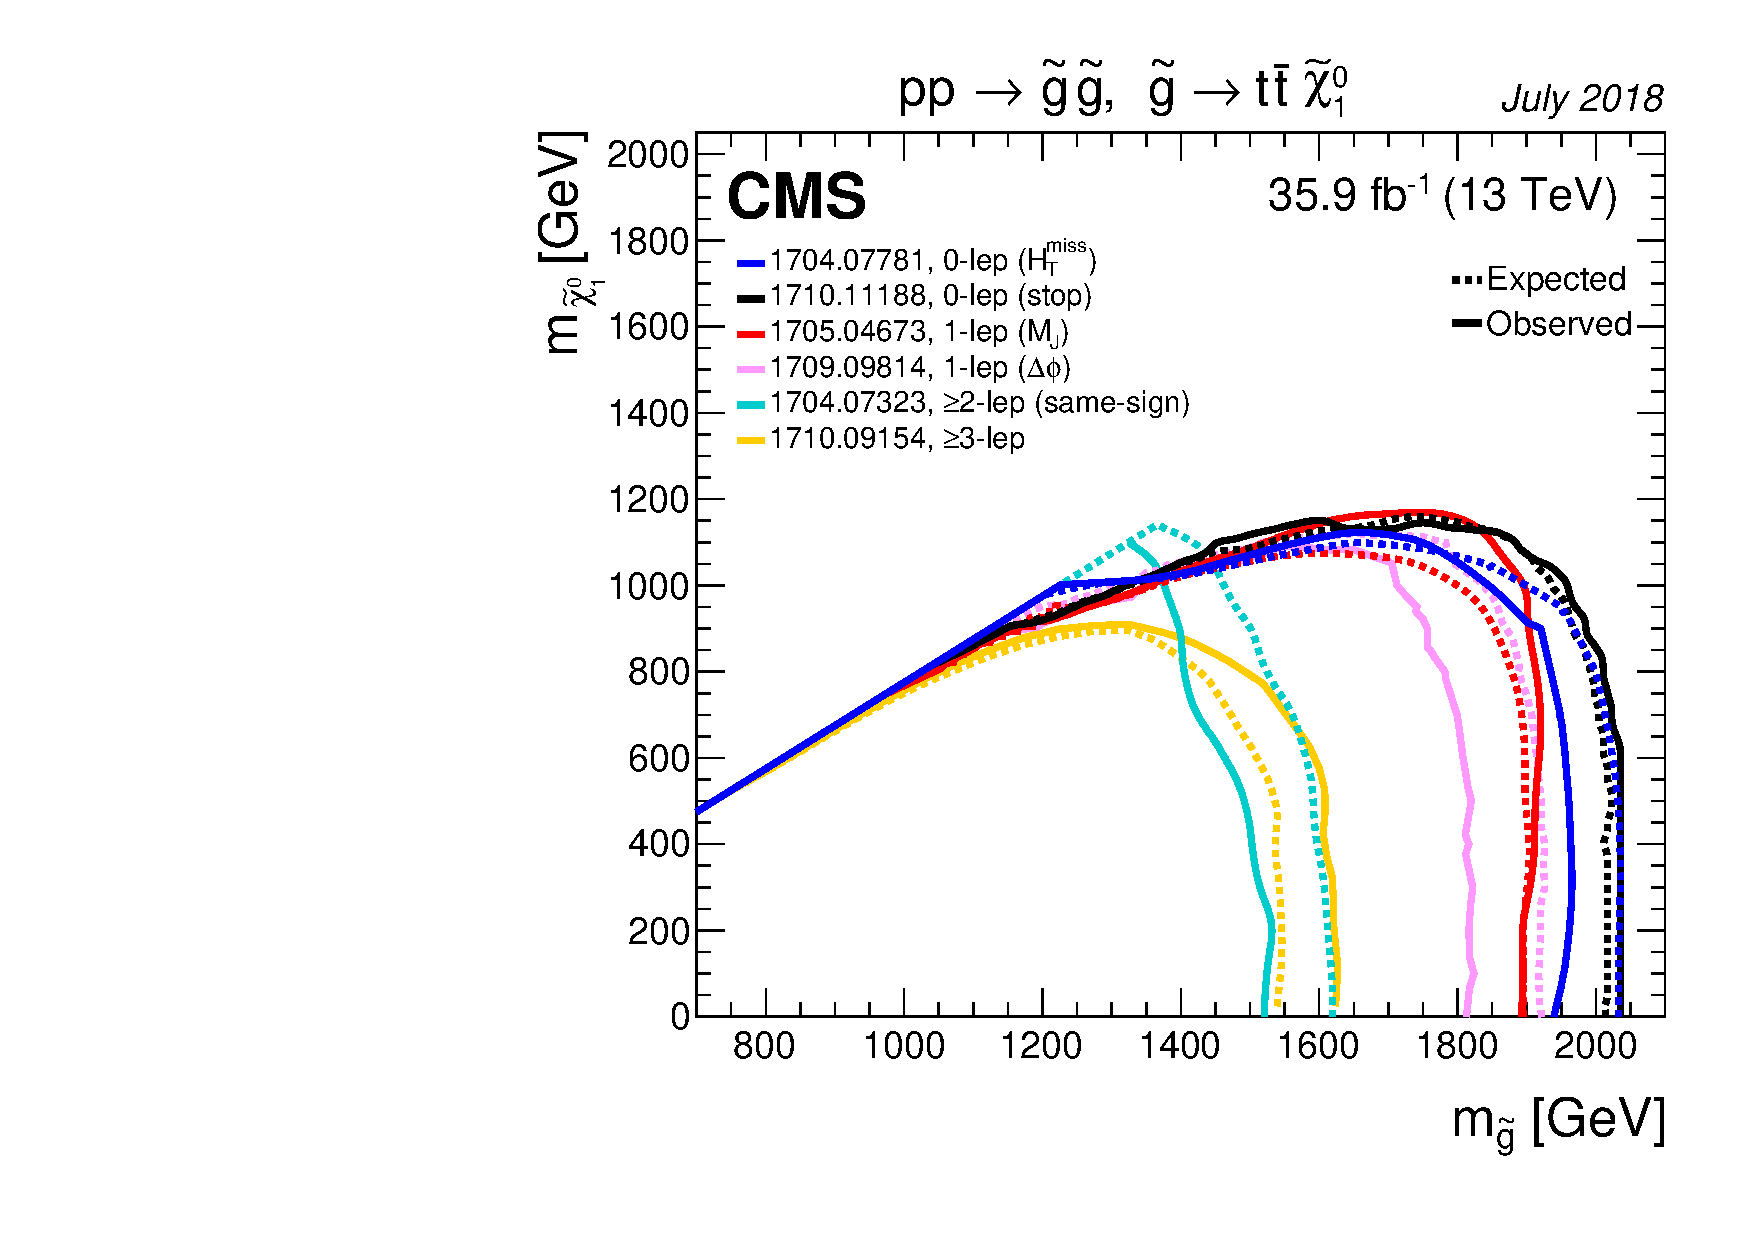
\includegraphics[width=0.49\textwidth]{figures/cms/T1tttt_limits_summary_cms.pdf}\label{fig:limits_Gtt_cms}}
	\subfigure[]{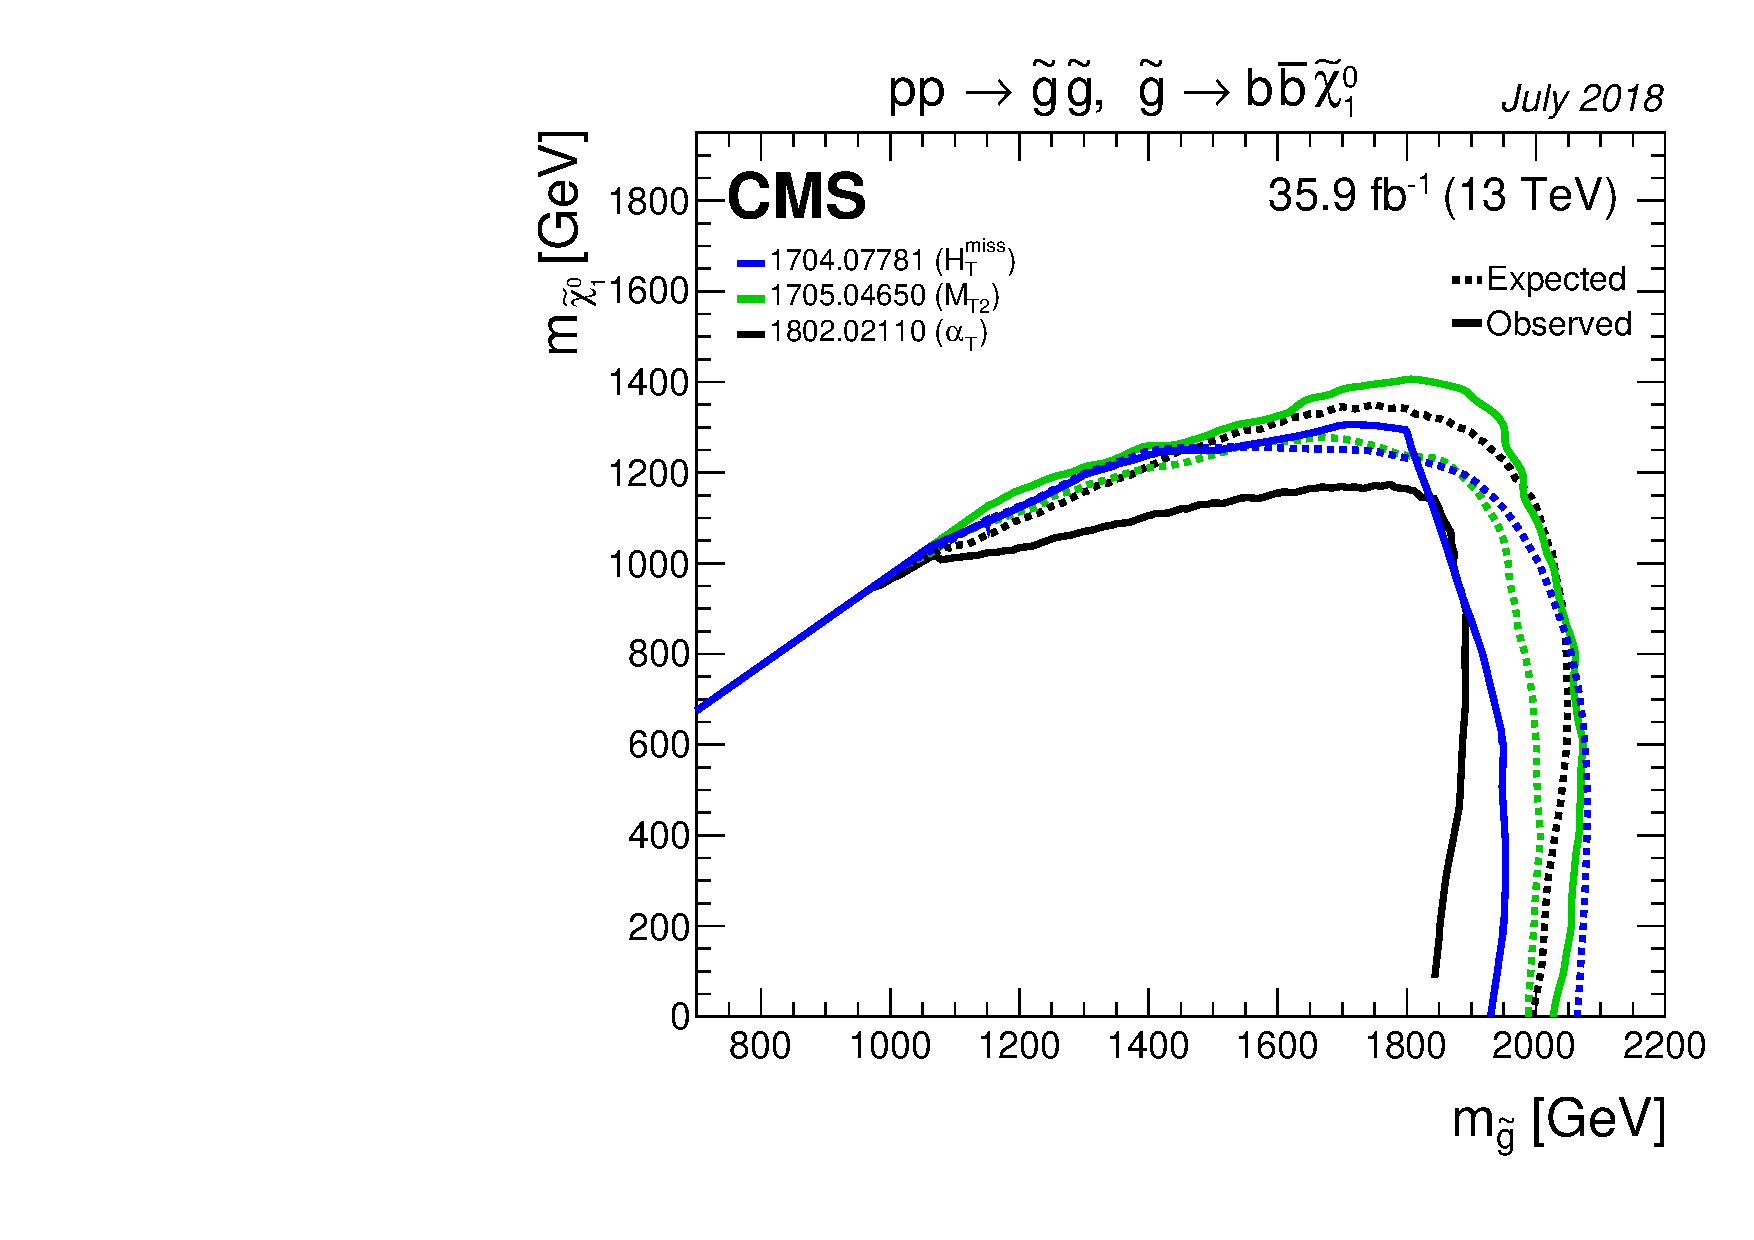
\includegraphics[width=0.49\textwidth]{figures/cms/T1bbbb_limits_summary_cms.pdf}\label{fig:limits_Gbb_cms}}
	\caption{Mass limits at 95\% CL obtained for simplified models of gluino pair production 
	with gluino decays to \subref{fig:limits_Gtt_cms} pairs of top quarks and the LSP and \subref{fig:limits_Gbb_cms}
	pairs of bottom quarks and the LSP. 
	In the figures, the solid (dashed) 
	lines correspond to the observed (median expected) limits. The arXiv numbers corresponding to the different analyses are shown in the legend.
	}
	\label{fig:limits_GbbGtt_comp}
\end{figure}

If we compare the \gls{atlas} and \gls{cms} results for this signal model, 
they overall provide similar sensitivity. 
For the Gtt signal, the \gls{atlas} multi-b analysis has an expected sensitivity about 100 GeV better than \gls{cms}, while 
for the Gbb model the \htmiss analysis extends the sensitivity of the multi-b analysis by about 50 GeV.

\FloatBarrier

\section{RPV interpretation}
\label{sec:rpvrpc}

Throughout this thesis, only models with R-parity conservation have been considered. 
The analysis presented in Chapter \ref{chap:strong_prod} is optimized for 
\gls{rpcsusy} scenarios, but it maintains some sensitivity also when \gls{rpv} couplings are considered. 
This has been studies in Ref. \cite{ATLAS-CONF-2018-003}, where several \gls{atlas} \gls{susy} analyses 
are reinterpreted in models with variable \gls{rpv} coupling strength.

In \gls{rpcsusy} models the \gls{lsp} is stable and, if it is neutral (as in the case of a \ninoone \gls{lsp} 
considered in the Gtt model) it escapes undetected, giving rise to final states rich in \met. 
This is no longer the case if we allow the presence of \gls{rpv} couplings: with the increase of the 
coupling strength, the \gls{lsp} goes from being long-lived, to having displaced decay vertices to 
having a prompt decay. 

In particular, in the case of the Gtt model, a non-zero $\lambda''_{323}$ coupling opens the decay 
$\ninoone \rightarrow t b s$, and large values  of $\lambda''_{323}$ can also lead to the 
direct decay $\tilde{g} \rightarrow t b s$. The different decay modes for various values of  
$\lambda''_{323}$ are shown in the diagrams in Figure \ref{fig:rpcrpv_diagrams}.
 

\begin{figure}[htbp]
	\centering 
	\subfigure[]{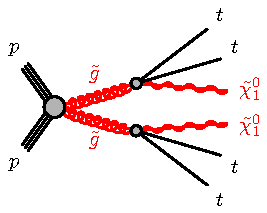
\includegraphics[width=0.32\textwidth]{figures/rpv/fig_01d.pdf}}
	\subfigure[]{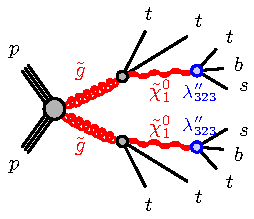
\includegraphics[width=0.32\textwidth]{figures/rpv/fig_01e.pdf}}
	\subfigure[]{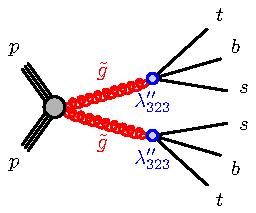
\includegraphics[width=0.32\textwidth]{figures/rpv/fig_01f.pdf}}
	\caption{Production and decay process for the \gls{rpv} Gtt model considered.
	 The dominant process varies with increasing $\lambda''_{323}$ coupling from left to right.}
	\label{fig:rpcrpv_diagrams}
\end{figure}

\begin{figure}[htbp]
	\centering
	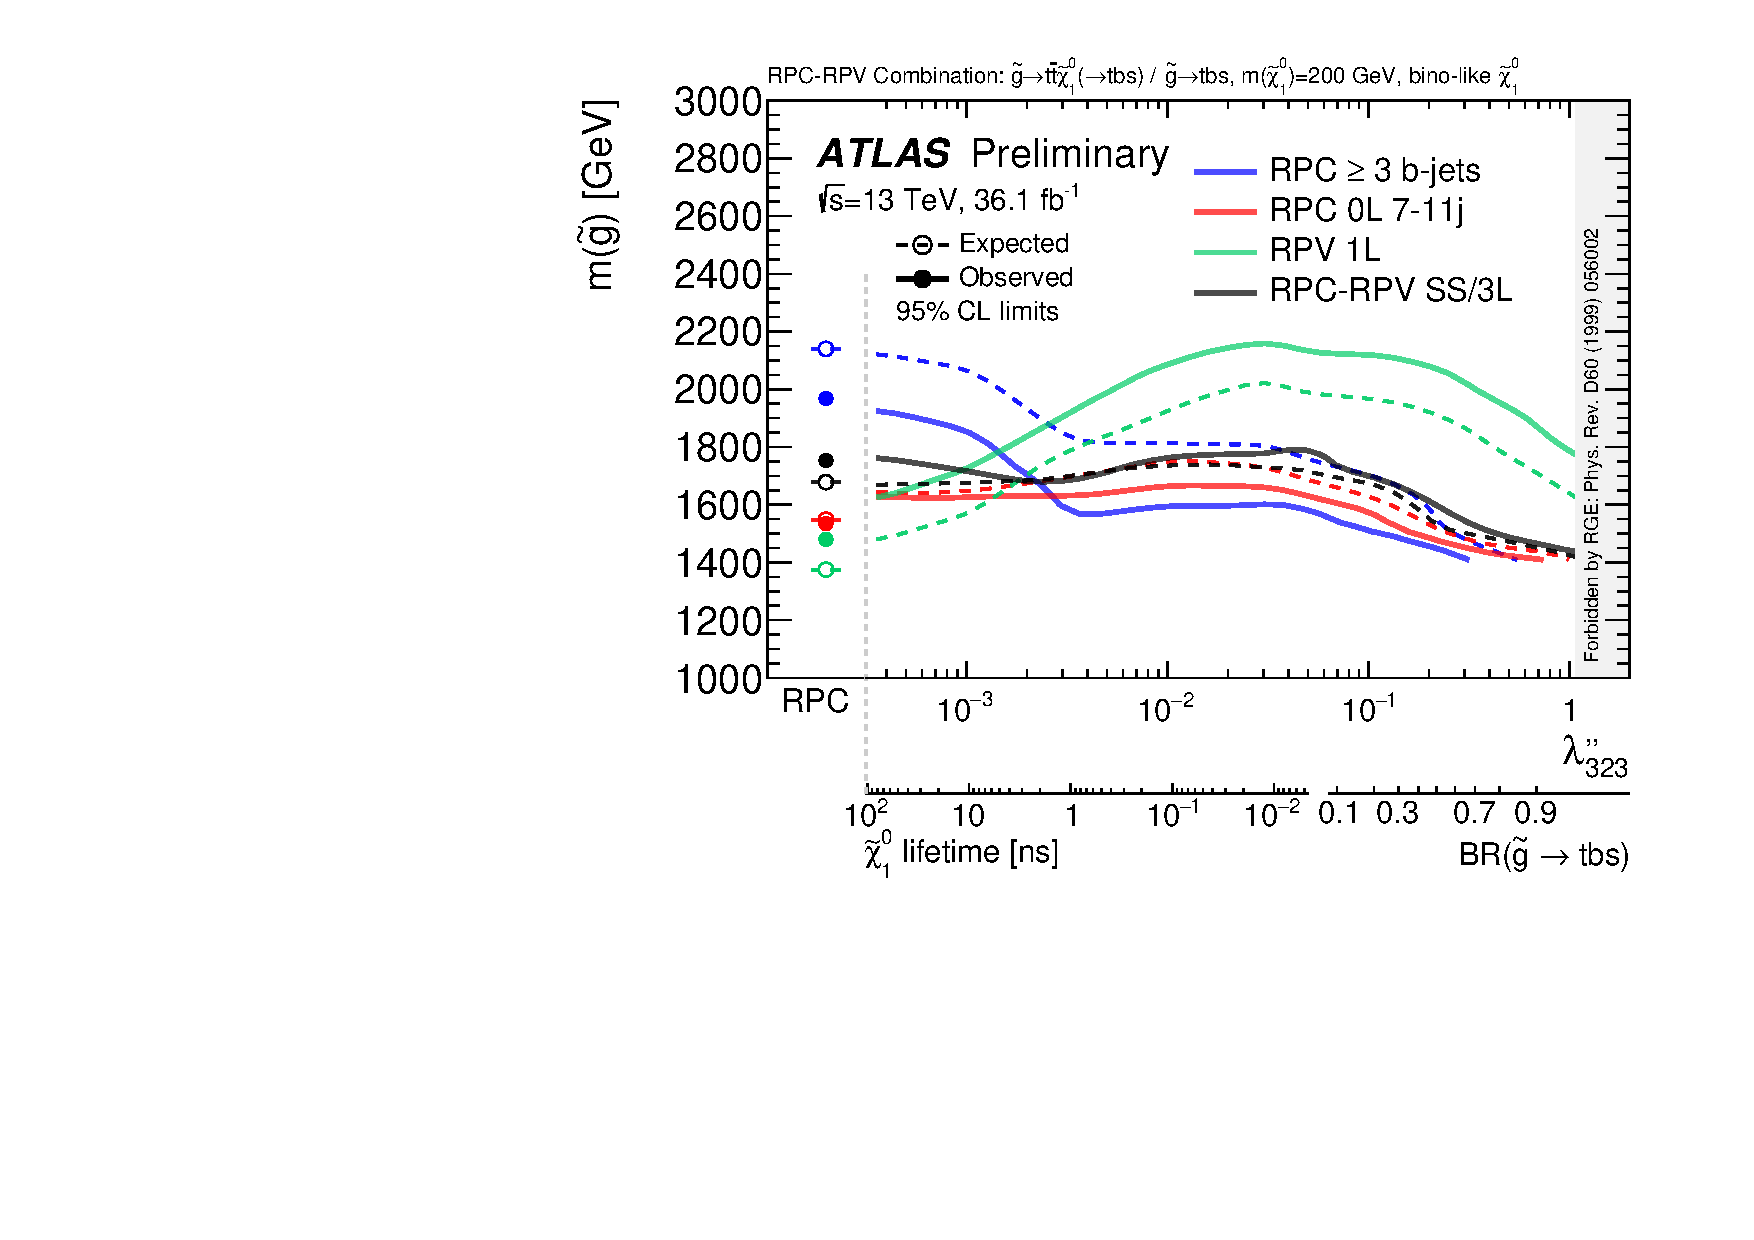
\includegraphics[width=0.63\textwidth]{figures/rpv/fig_04.pdf}
	\caption{	
	Exclusion limits for the Gtt model as a function of $\lambda_{323}''$ and m($\tilde{g}$). Expected limits are shown with dashed lines, and observed as solid. The \gls{rpcsusy}-limit is shown on the leftmost part of the axes, while the region $\lambda_{323}''>$ 1.07 is forbidden by constraints from the renormalization group equations. Figure from Ref. \cite{ATLAS-CONF-2018-003}.
	} 
	\label{fig:rpv_Gtt}
\end{figure}

The exclusion limit from the reinterpretation of four different \gls{atlas} searches, including the multi-b search, 
is shown in Figure \ref{fig:rpv_Gtt} in the m($\tilde{g}$)-$\lambda''_{323}$ plane, assuming m(\ninoone) = 200 GeV and  
m($\tilde{t}$/$\tilde{b}$) = 2.4 TeV. 
The multi-b search is the most sensitive for \ninoone lifetimes lower than 0.6 ns. 


\FloatBarrier

\section{Higgsino pair production in GMSB models}

The exclusion contours in the plane of \mhino-\gls{br} plane are shown in Figures \ref{fig:summary_atlas_higgsino_GMSB} 
and \ref{fig:limits_higgsino_cms} for the \gls{atlas} and \gls{cms} collaborations respectively.

The results included in Figure \ref{fig:summary_atlas_higgsino_GMSB} are the multi-b \met-based search described in Chapter \ref{chap:ewk_prod},
the low-mass multi-b search mentioned in Section \ref{sec:ewk:LM} and 
the four-lepton search presented in Ref. \cite{Aaboud:2018zeb}, that requires two pairs of same-sign opposite-flavor leptons 
with invariant mass compatible with a Z boson, and defines two \glspl{sr} to target \gls{gmsb} higgsino pair production, respectively 
with a 50 GeV and 100 GeV \met requirement. This search is by construction more sensitive to models with a high $B(\hino\rightarrow Z \tilde{G})$.

\begin{figure}[htbp]
	\centering
	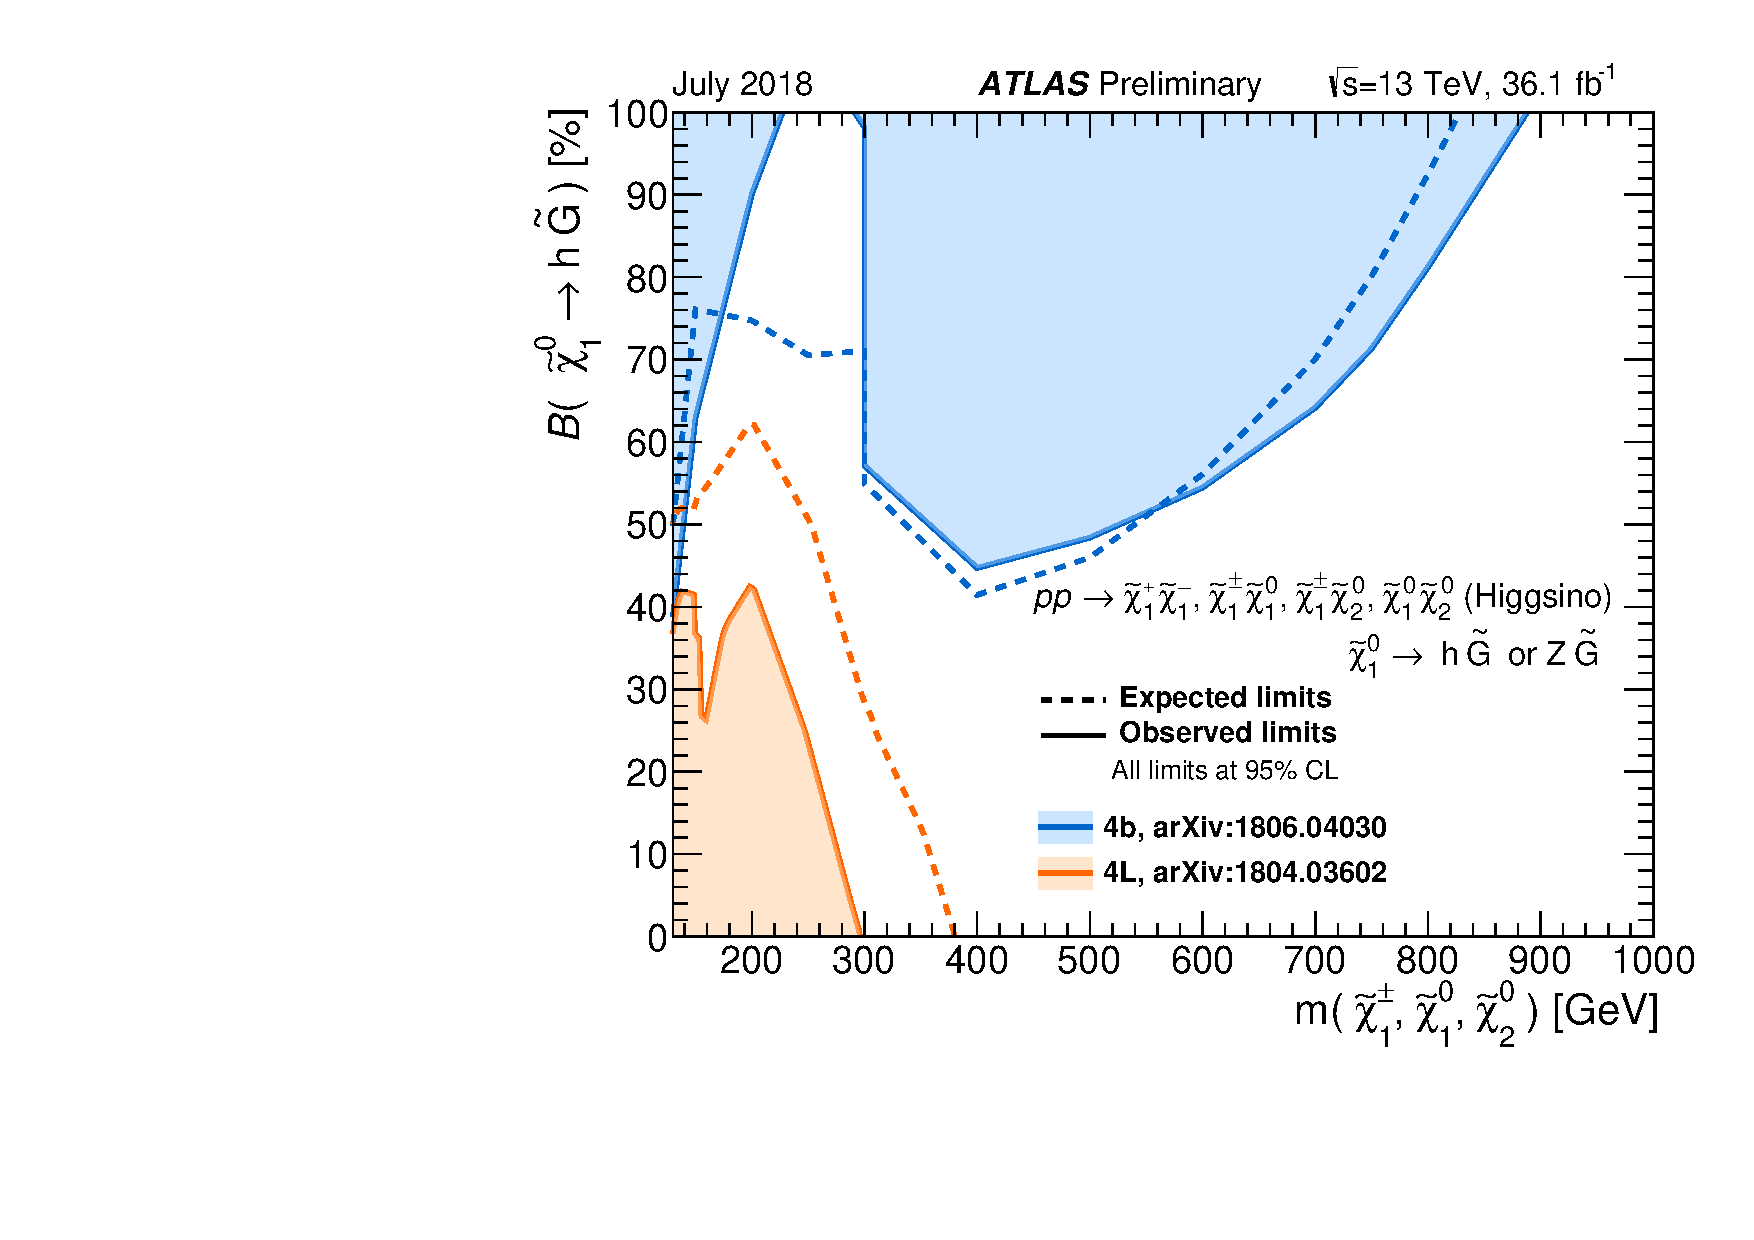
\includegraphics[width=0.65\textwidth]{figures/summary_plots/ATLAS_SUSY_EWSummary_GGM.pdf}
	\caption{The 95\% CL exclusion limits on a general gauge mediation model from 13 TeV data. 
	The model assumes a pure Higgsino NLSP that promptly decays to either Z gravitino or Higgs gravitino. 
	The limits are displayed as a function of the mass of the nearly mass-degenerate Higgsino triplet and the branching fraction of lightest Higgsino to Higgs gravitino. 	Figure from Ref. \cite{atlasSUSYSummary}.
	} 
	\label{fig:summary_atlas_higgsino_GMSB}
\end{figure}

The \gls{cms} collaboration has a more extensive program covering this signal model for what concerns the analysis of the 
2015-2016 dataset. 
Different final states are exploited to be sensitive to the possible combinations of branching ratios, 
providing a good sensitivity throughout the full plane.
Figure \ref{fig:limits_higgsino_cms_comb} shows the combined exclusion contour: the expected sensitivity is up to about 580 GeV in the case $B(\hino\rightarrow Z \tilde{G})=100$\% and 800 GeV for 
$B(\hino\rightarrow h \tilde{G})=100$\%.

\begin{figure}[htbp]
	\centering 
	\subfigure[]{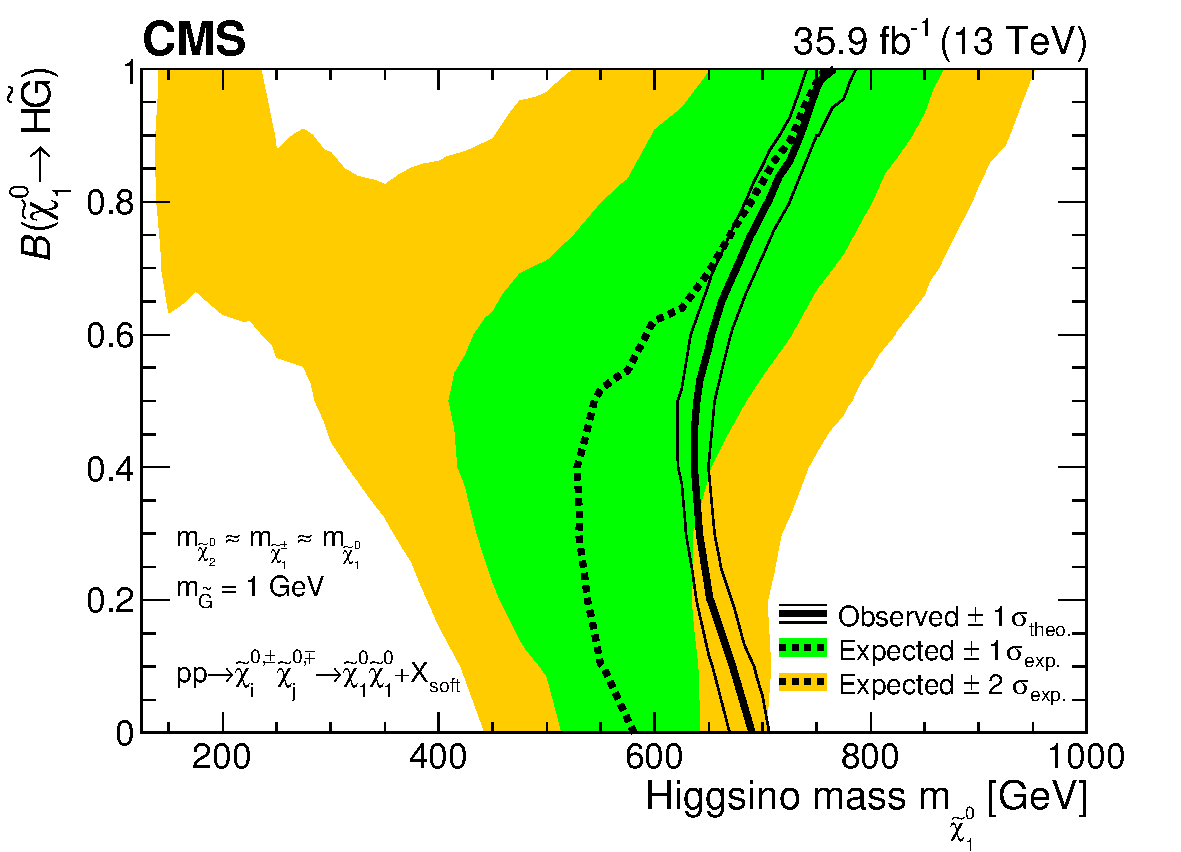
\includegraphics[width=0.49\textwidth]{figures/cms/CMS-SUS-17-004_Figure_011.pdf}\label{fig:limits_higgsino_cms_comb}}
	\subfigure[]{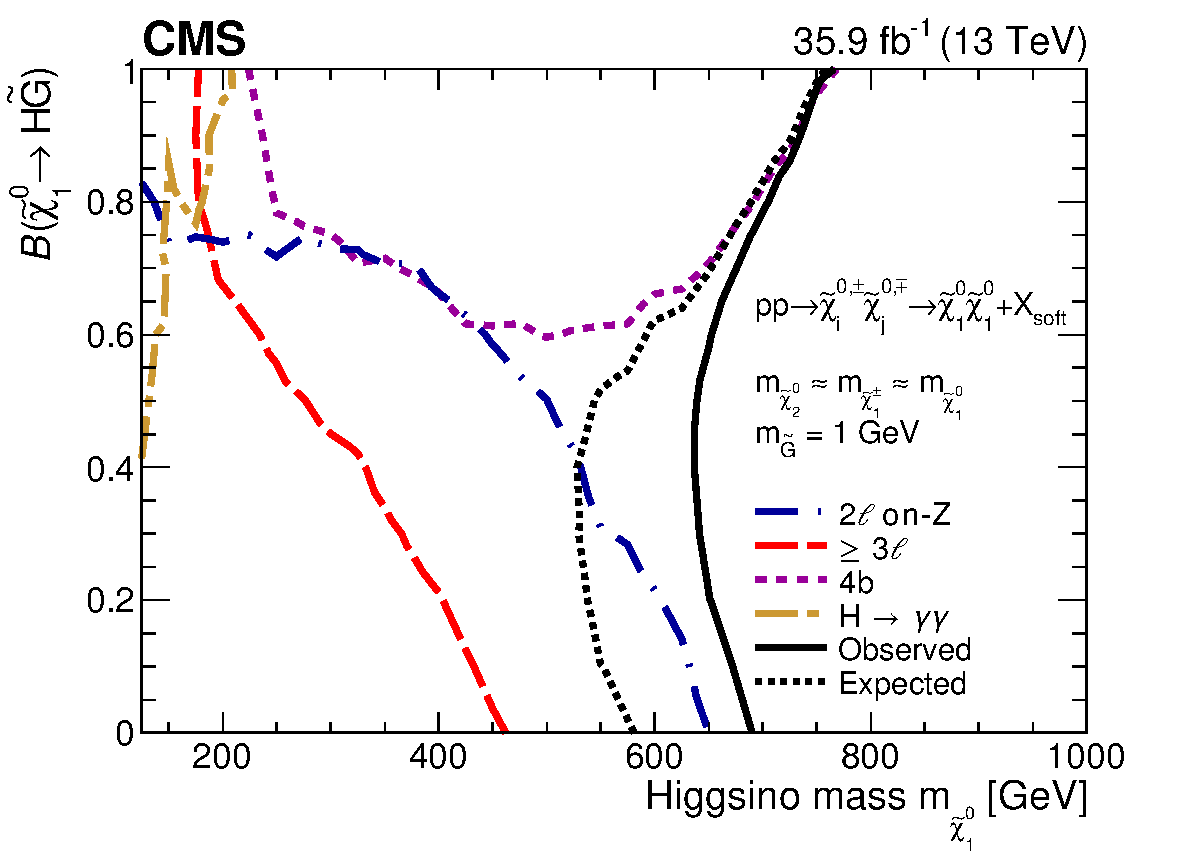
\includegraphics[width=0.49\textwidth]{figures/cms/CMS-SUS-17-004_Figure_012.pdf}\label{fig:limits_higgsino_cms_individual}}
	\caption{
	Exclusion contours at the 95\% CL in the plane of m(\ninoone) and \gls{br}(\ninoone $\to$ H \gravino) for the model of \ninoone\ninoone production.
    \subref{fig:limits_higgsino_cms_comb}     
	Combined exclusion contours. The area to the left of or below the solid (dashed) black curve represents the observed (expected) exclusion region. The green and yellow bands indicate the $\pm1$ and $2\sigma$ uncertainties in the expected limit. The thin black lines show the effect of the theoretical uncertainties ($\pm1\sigma_{theory}$) on the signal cross section.
	\subref{fig:limits_higgsino_cms_individual}
	Observed contours for each individual analysis compared with the combination. For the 4b contour, the region above is excluded, while for all others, the region to the left is excluded. The 4b search drives the exclusion at large values of \gls{br}(\ninoone $\to$ H \gravino) while the on-Z dilepton and multilepton searches are competing at lower values of \gls{br}(\ninoone $\to$ H \gravino).
	Figures from Ref. \cite{Sirunyan:2018ubx}.
		}
	\label{fig:limits_higgsino_cms}
\end{figure}

Figure \ref{fig:limits_higgsino_cms_individual} shows the observed exclusion limit for each individual analysis. 
We can see that, as it is the case for \gls{atlas}, the 4b search \cite{Sirunyan:2017obz} provides the 
best sensitivity for models with high $B(\hino\rightarrow h \tilde{G})$, except for low \mhino, where 
it is instead the two photons \cite{Sirunyan:2017eie} that provides the most stringent limit.
This is because the 4b analysis in \gls{cms} selects events that fire one of multiple triggers, 
all of which require some \met. 
Instead the \gls{atlas} analysis comprises also the low-mass part, that is very sensitive fro low \mhino.
The signals with intermediate and high $B(\hino\rightarrow Z \tilde{G})$ are probed with a 
search with two leptons consistent with the Z-boson peak \cite{Sirunyan:2017qaj}. 
\gls{atlas} at the moment does not have a 2-lepton search that provides a good sensitivity to this model,
and therefore had overall a less good coverage of the \mhino-\gls{br} plane.
Despite this, the comparison of the \gls{cms} 4b search with the multi-b search from \gls{atlas}
described in Chapter \ref{chap:ewk_prod} shows a better sensitivity of the \gls{atlas} search, 
especially at high Higgsino mass,
where the very low background regions of the \gls{atlas} analysis provides better sensitivity. 

%three-lepton search \cite{Sirunyan:2017lae}



\FloatBarrier


\section{ATLAS mass reach}

\begin{figure}[htb]
	\centering
	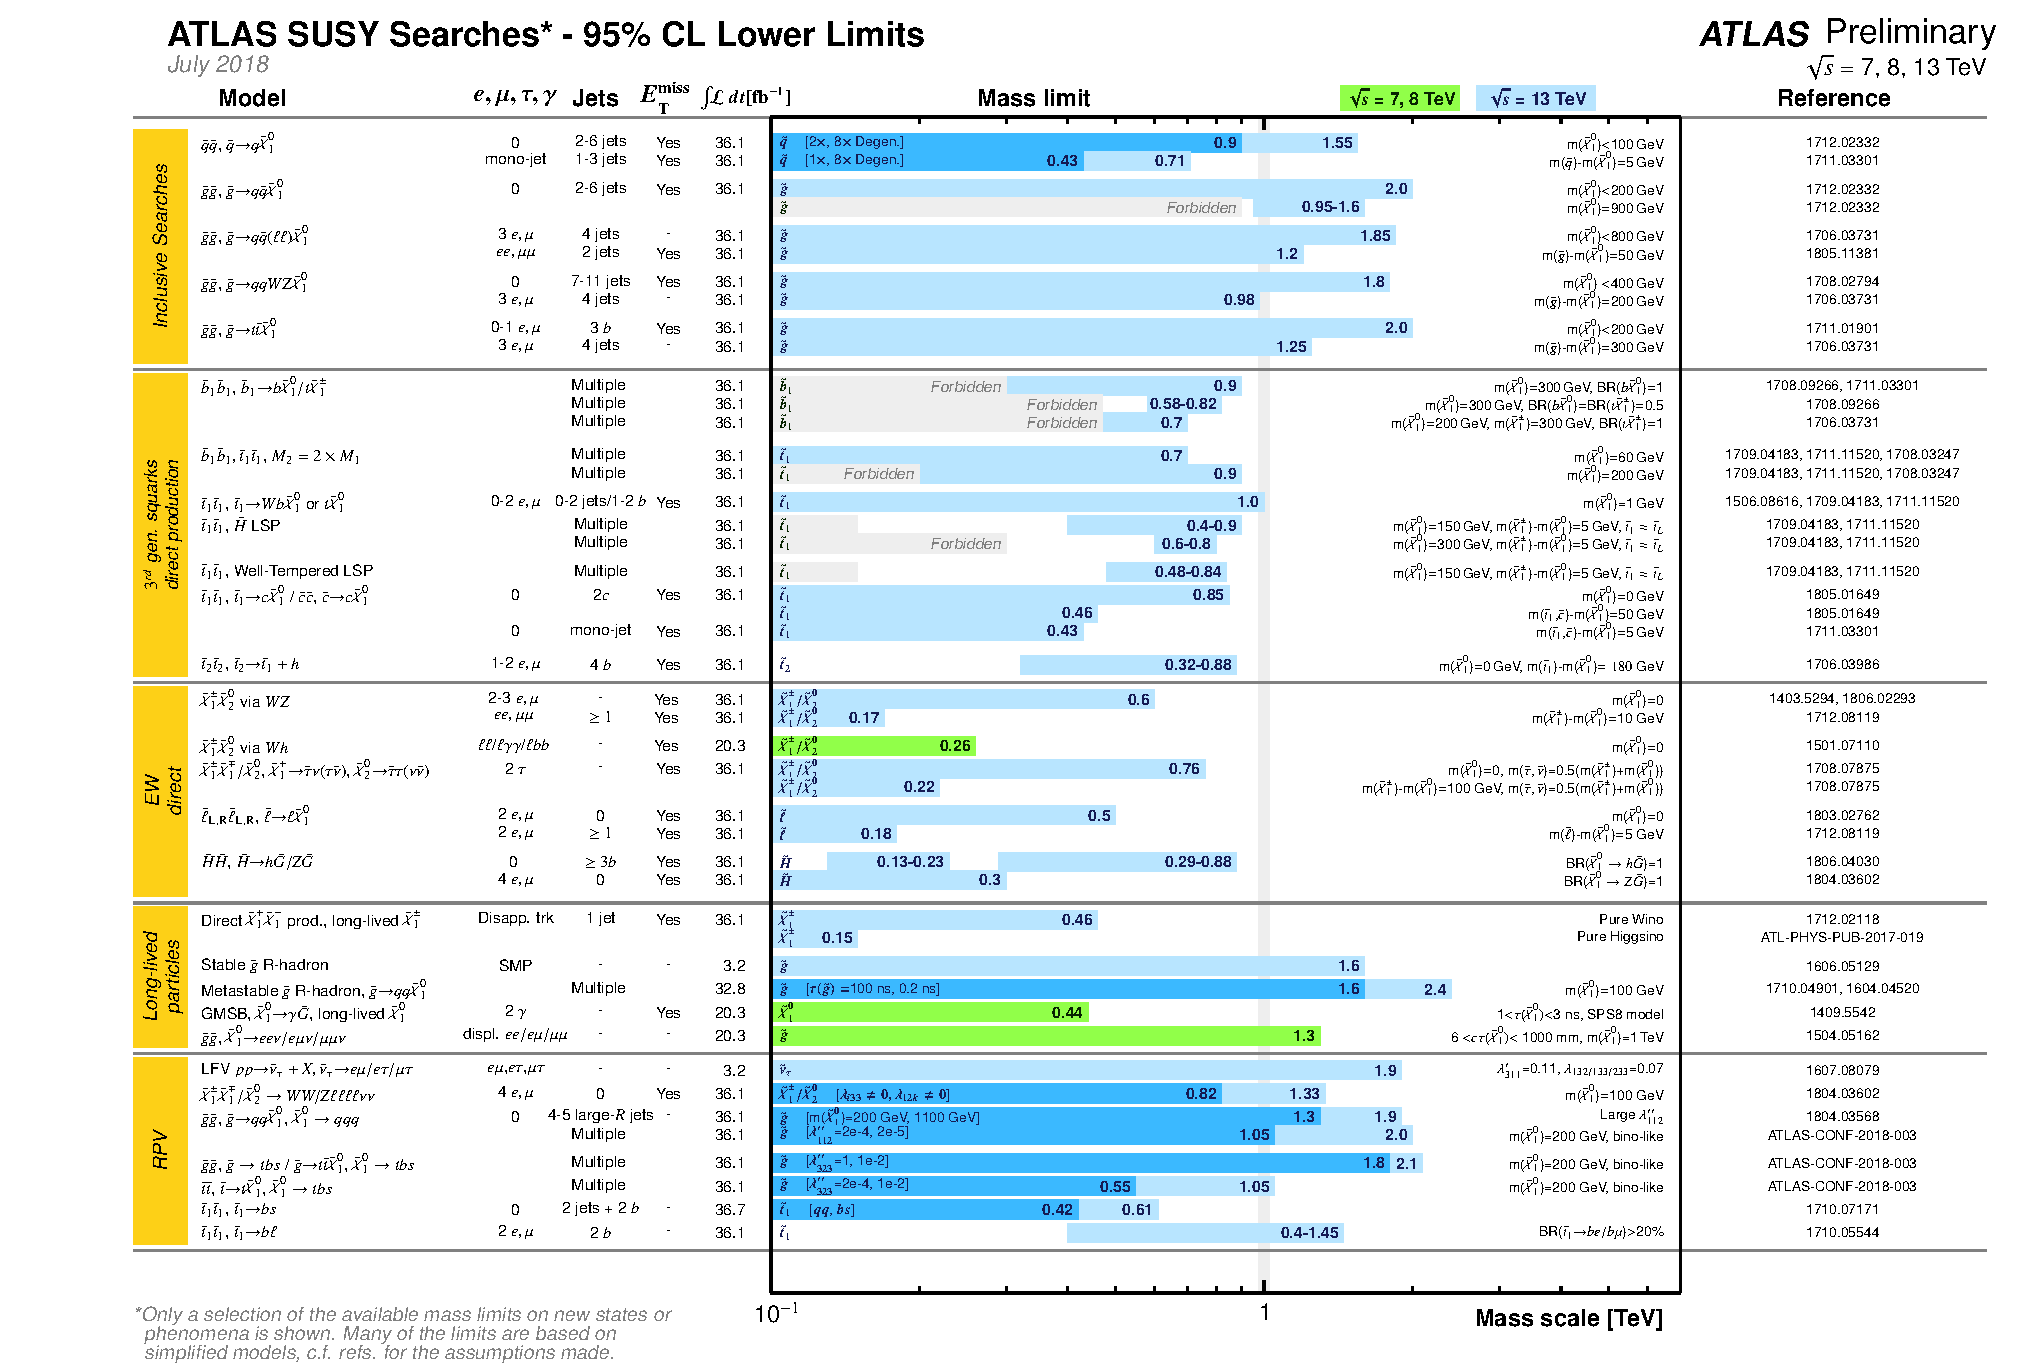
\includegraphics[width=1.1\textwidth]{figures/summary_plots/ATLAS_SUSY_Summary.pdf}
	\caption{Mass reach of the ATLAS searches for Supersymmetry. 
	A representative selection of the available search results is shown. Results are quoted for the nominal cross section 
	in both a region of near-maximal mass reach and a demonstrative alternative scenario, in order to display the range in 
	model space of search sensitivity. Some limits depend on additional assumptions on the mass of the intermediate states, 
	as described in the references provided in the plot. Figure from Ref. \cite{atlasSUSYSummary}.
	} 
	\label{fig:summary_atlas_summary}
\end{figure}

Figure \ref{fig:summary_atlas_summary} shows the mass reach of the \gls{atlas} \gls{susy} searches on 
some representative signal models, as of July 2018. 
Signal models are divided by production mode and/or model assumptions into:
\begin{description}

\item[Inclusive searches] Analyses that look for direct production of squarks (except 3$^{rd}$ generation squarks)
and gluinos, including the strong-production multi-b analysis, are grouped into this category. For the multi-b analysis,
only the Gtt result is reported. The assumptions of this model lead to a spectacular final state, rich in jets and b-jets, that 
allow us to effectively separate signal from background, leading to the gluino mass limit of 2 TeV for low neutralino mass.
This should not be translated into the universal statement that gluinos with mass of 2 TeV are excluded: 
as it has already been noticed in Chapter \ref{chap:strong_prod}, an higher neutralino mass weakens substantially the observed limit.
From Figure \ref{fig:summary_atlas_summary} we can further learn that the assumptions on the gluino decay mode can alter the limits as well,
and in fact the all the limits are weaker than the ones we obtain for decays to third generation particles.

\item[3$^{rd}$ generation squark direct production] In natural \gls{susy} models third generation squarks are expected to be 
relatively light, and this motivates the extensive \gls{atlas} program to search for stop and sbottom production. 
Also in this case, Figure \ref{fig:summary_atlas_summary} shows how the limits set by the different analyses depend a lot from the 
decay mode assumed; for example, in the case of m($\tilde{t}_1$), the observed limits range from 430 GeV in the case of a decay 
to the charm quark to up to 1 TeV if the decay is instead to a top quark.

\item[EW direct] The direct production of charginos, neutralinos and sleptons has the lowest limits due to the lower electroweak
production cross section compared to processes mediated by the strong force. The strongest mass limit is places by the multi-b 
electroweak analysis, that excludes Higgisnos up to 880 GeV. This wide exclusion range compared to the other electroweak analyses
is due to the peculiar features of the final state and to the large Higgsino cross section (four different production modes that are equivalent 
because of the degeneracy of \ninoone, \ninotwo, \chinoonepm). 

\item[Long-lived particles] The analyses discussed in this thesis, as well as the models mentioned in the three points above, assume that 
all \gls{susy} particles originate a chain of prompt decays to \gls{sm} particles and the \gls{lsp}.
Including in the signal models a non-zero lifetime for \gls{susy} particles leads to very different signatures that can be exploited to 
search for \gls{bsm} physics. In this case the range of exclusion depends on the lifetime itself, and in 
favorable cases it can lead to stronger bounds than the ones obtained for prompt decays;
this is the case for example for gluinos decaying to light quarks, that are excluded up to 2.4 TeV for a gluino lifetime of 0.2 ns.  

\item[RPV] The reason why a large number of the \gls{atlas} \gls{susy} searches require the presence of \met is that in R-parity conserving models 
the \gls{lsp} is long lived and therefore, if it has zero charge, it escapes detection. In \gls{rpv} models this is no longer the case,
and the final states have less \met (originating only from neutrinos form \gls{sm} decays) and in general more visible decay products. 
The limits placed in the case of \gls{rpv} models are similar or larges than the ones places for corresponding \gls{rpcsusy} scenarios, as it is 
the case e.g. for the $\tilde{t}_1$, excluded between 400 GeV and 1.45 TeV if the $B-L$-conserving decay $\tilde{t}_1 \to b l$ is allowed. 
As already discussed in Section \ref{sec:rpvrpc}, the strength of the \gls{rpv} couplings can change noticeably the sensitivity of the 
analyses. 

\end{description}

